
%% bare_conf.tex
%% V1.4b
%% 2015/08/26
%% by Michael Shell
%% See:
%% http://www.michaelshell.org/
%% for current contact information.
%%
%% This is a skeleton file demonstrating the use of IEEEtran.cls
%% (requires IEEEtran.cls version 1.8b or later) with an IEEE
%% conference paper.
%%
%% Support sites:
%% http://www.michaelshell.org/tex/ieeetran/
%% http://www.ctan.org/pkg/ieeetran
%% and
%% http://www.ieee.org/

%%*************************************************************************
%% Legal Notice:
%% This code is offered as-is without any warranty either expressed or
%% implied; without even the implied warranty of MERCHANTABILITY or
%% FITNESS FOR A PARTICULAR PURPOSE! 
%% User assumes all risk.
%% In no event shall the IEEE or any contributor to this code be liable for
%% any damages or losses, including, but not limited to, incidental,
%% consequential, or any other damages, resulting from the use or misuse
%% of any information contained here.
%%
%% All comments are the opinions of their respective authors and are not
%% necessarily endorsed by the IEEE.
%%
%% This work is distributed under the LaTeX Project Public License (LPPL)
%% ( http://www.latex-project.org/ ) version 1.3, and may be freely used,
%% distributed and modified. A copy of the LPPL, version 1.3, is included
%% in the base LaTeX documentation of all distributions of LaTeX released
%% 2003/12/01 or later.
%% Retain all contribution notices and credits.
%% ** Modified files should be clearly indicated as such, including  **
%% ** renaming them and changing author support contact information. **
%%*************************************************************************


% *** Authors should verify (and, if needed, correct) their LaTeX system  ***
% *** with the testflow diagnostic prior to trusting their LaTeX platform ***
% *** with production work. The IEEE's font choices and paper sizes can   ***
% *** trigger bugs that do not appear when using other class files.       ***                          ***
% The testflow support page is at:
% http://www.michaelshell.org/tex/testflow/



\documentclass[conference]{IEEEtran}
\usepackage{lmodern}
\usepackage[T1]{fontenc}
\usepackage{textcomp}
\usepackage[utf8]{inputenc}
\usepackage{graphicx}
\usepackage{subfigure}
\usepackage{amsmath} % assumes amsmath package installed
\usepackage{amssymb} 
\usepackage{array}

\usepackage{blindtext}
\usepackage{color}

% Some Computer Society conferences also require the compsoc mode option,
% but others use the standard conference format.
%
% If IEEEtran.cls has not been installed into the LaTeX system files,
% manually specify the path to it like:
% \documentclass[conference]{../sty/IEEEtran}





% Some very useful LaTeX packages include:
% (uncomment the ones you want to load)


% *** MISC UTILITY PACKAGES ***
%
%\usepackage{ifpdf}
% Heiko Oberdiek's ifpdf.sty is very useful if you need conditional
% compilation based on whether the output is pdf or dvi.
% usage:
% \ifpdf
%   % pdf code
% \else
%   % dvi code
% \fi
% The latest version of ifpdf.sty can be obtained from:
% http://www.ctan.org/pkg/ifpdf
% Also, note that IEEEtran.cls V1.7 and later provides a builtin
% \ifCLASSINFOpdf conditional that works the same way.
% When switching from latex to pdflatex and vice-versa, the compiler may
% have to be run twice to clear warning/error messages.






% *** CITATION PACKAGES ***
%
%\usepackage{cite}
% cite.sty was written by Donald Arseneau
% V1.6 and later of IEEEtran pre-defines the format of the cite.sty package
% \cite{} output to follow that of the IEEE. Loading the cite package will
% result in citation numbers being automatically sorted and properly
% "compressed/ranged". e.g., [1], [9], [2], [7], [5], [6] without using
% cite.sty will become [1], [2], [5]--[7], [9] using cite.sty. cite.sty's
% \cite will automatically add leading space, if needed. Use cite.sty's
% noadjust option (cite.sty V3.8 and later) if you want to turn this off
% such as if a citation ever needs to be enclosed in parenthesis.
% cite.sty is already installed on most LaTeX systems. Be sure and use
% version 5.0 (2009-03-20) and later if using hyperref.sty.
% The latest version can be obtained at:
% http://www.ctan.org/pkg/cite
% The documentation is contained in the cite.sty file itself.






% *** GRAPHICS RELATED PACKAGES ***
%
\ifCLASSINFOpdf
  % \usepackage[pdftex]{graphicx}
  % declare the path(s) where your graphic files are
  % \graphicspath{{../pdf/}{../jpeg/}}
  % and their extensions so you won't have to specify these with
  % every instance of \includegraphics
  % \DeclareGraphicsExtensions{.pdf,.jpeg,.png}
\else
  % or other class option (dvipsone, dvipdf, if not using dvips). graphicx
  % will default to the driver specified in the system graphics.cfg if no
  % driver is specified.
  % \usepackage[dvips]{graphicx}
  % declare the path(s) where your graphic files are
  % \graphicspath{{../eps/}}
  % and their extensions so you won't have to specify these with
  % every instance of \includegraphics
  % \DeclareGraphicsExtensions{.eps}
\fi
% graphicx was written by David Carlisle and Sebastian Rahtz. It is
% required if you want graphics, photos, etc. graphicx.sty is already
% installed on most LaTeX systems. The latest version and documentation
% can be obtained at: 
% http://www.ctan.org/pkg/graphicx
% Another good source of documentation is "Using Imported Graphics in
% LaTeX2e" by Keith Reckdahl which can be found at:
% http://www.ctan.org/pkg/epslatex
%
% latex, and pdflatex in dvi mode, support graphics in encapsulated
% postscript (.eps) format. pdflatex in pdf mode supports graphics
% in .pdf, .jpeg, .png and .mps (metapost) formats. Users should ensure
% that all non-photo figures use a vector format (.eps, .pdf, .mps) and
% not a bitmapped formats (.jpeg, .png). The IEEE frowns on bitmapped formats
% which can result in "jaggedy"/blurry rendering of lines and letters as
% well as large increases in file sizes.
%
% You can find documentation about the pdfTeX application at:
% http://www.tug.org/applications/pdftex





% *** MATH PACKAGES ***
%
%\usepackage{amsmath}
% A popular package from the American Mathematical Society that provides
% many useful and powerful commands for dealing with mathematics.
%
% Note that the amsmath package sets \interdisplaylinepenalty to 10000
% thus preventing page breaks from occurring within multiline equations. Use:
%\interdisplaylinepenalty=2500
% after loading amsmath to restore such page breaks as IEEEtran.cls normally
% does. amsmath.sty is already installed on most LaTeX systems. The latest
% version and documentation can be obtained at:
% http://www.ctan.org/pkg/amsmath





% *** SPECIALIZED LIST PACKAGES ***
%
%\usepackage{algorithmic}
% algorithmic.sty was written by Peter Williams and Rogerio Brito.
% This package provides an algorithmic environment fo describing algorithms.
% You can use the algorithmic environment in-text or within a figure
% environment to provide for a floating algorithm. Do NOT use the algorithm
% floating environment provided by algorithm.sty (by the same authors) or
% algorithm2e.sty (by Christophe Fiorio) as the IEEE does not use dedicated
% algorithm float types and packages that provide these will not provide
% correct IEEE style captions. The latest version and documentation of
% algorithmic.sty can be obtained at:
% http://www.ctan.org/pkg/algorithms
% Also of interest may be the (relatively newer and more customizable)
% algorithmicx.sty package by Szasz Janos:
% http://www.ctan.org/pkg/algorithmicx




% *** ALIGNMENT PACKAGES ***
%
%\usepackage{array}
% Frank Mittelbach's and David Carlisle's array.sty patches and improves
% the standard LaTeX2e array and tabular environments to provide better
% appearance and additional user controls. As the default LaTeX2e table
% generation code is lacking to the point of almost being broken with
% respect to the quality of the end results, all users are strongly
% advised to use an enhanced (at the very least that provided by array.sty)
% set of table tools. array.sty is already installed on most systems. The
% latest version and documentation can be obtained at:
% http://www.ctan.org/pkg/array


% IEEEtran contains the IEEEeqnarray family of commands that can be used to
% generate multiline equations as well as matrices, tables, etc., of high
% quality.




% *** SUBFIGURE PACKAGES ***
%\ifCLASSOPTIONcompsoc
%  \usepackage[caption=false,font=normalsize,labelfont=sf,textfont=sf]{subfig}
%\else
%  \usepackage[caption=false,font=footnotesize]{subfig}
%\fi
% subfig.sty, written by Steven Douglas Cochran, is the modern replacement
% for subfigure.sty, the latter of which is no longer maintained and is
% incompatible with some LaTeX packages including fixltx2e. However,
% subfig.sty requires and automatically loads Axel Sommerfeldt's caption.sty
% which will override IEEEtran.cls' handling of captions and this will result
% in non-IEEE style figure/table captions. To prevent this problem, be sure
% and invoke subfig.sty's "caption=false" package option (available since
% subfig.sty version 1.3, 2005/06/28) as this is will preserve IEEEtran.cls
% handling of captions.
% Note that the Computer Society format requires a larger sans serif font
% than the serif footnote size font used in traditional IEEE formatting
% and thus the need to invoke different subfig.sty package options depending
% on whether compsoc mode has been enabled.
%
% The latest version and documentation of subfig.sty can be obtained at:
% http://www.ctan.org/pkg/subfig




% *** FLOAT PACKAGES ***
%
%\usepackage{fixltx2e}
% fixltx2e, the successor to the earlier fix2col.sty, was written by
% Frank Mittelbach and David Carlisle. This package corrects a few problems
% in the LaTeX2e kernel, the most notable of which is that in current
% LaTeX2e releases, the ordering of single and double column floats is not
% guaranteed to be preserved. Thus, an unpatched LaTeX2e can allow a
% single column figure to be placed prior to an earlier double column
% figure.
% Be aware that LaTeX2e kernels dated 2015 and later have fixltx2e.sty's
% corrections already built into the system in which case a warning will
% be issued if an attempt is made to load fixltx2e.sty as it is no longer
% needed.
% The latest version and documentation can be found at:
% http://www.ctan.org/pkg/fixltx2e


%\usepackage{stfloats}
% stfloats.sty was written by Sigitas Tolusis. This package gives LaTeX2e
% the ability to do double column floats at the bottom of the page as well
% as the top. (e.g., "\begin{figure*}[!b]" is not normally possible in
% LaTeX2e). It also provides a command:
%\fnbelowfloat
% to enable the placement of footnotes below bottom floats (the standard
% LaTeX2e kernel puts them above bottom floats). This is an invasive package
% which rewrites many portions of the LaTeX2e float routines. It may not work
% with other packages that modify the LaTeX2e float routines. The latest
% version and documentation can be obtained at:
% http://www.ctan.org/pkg/stfloats
% Do not use the stfloats baselinefloat ability as the IEEE does not allow
% \baselineskip to stretch. Authors submitting work to the IEEE should note
% that the IEEE rarely uses double column equations and that authors should try
% to avoid such use. Do not be tempted to use the cuted.sty or midfloat.sty
% packages (also by Sigitas Tolusis) as the IEEE does not format its papers in
% such ways.
% Do not attempt to use stfloats with fixltx2e as they are incompatible.
% Instead, use Morten Hogholm'a dblfloatfix which combines the features
% of both fixltx2e and stfloats:
%
% \usepackage{dblfloatfix}
% The latest version can be found at:
% http://www.ctan.org/pkg/dblfloatfix




% *** PDF, URL AND HYPERLINK PACKAGES ***
%
%\usepackage{url}
% url.sty was written by Donald Arseneau. It provides better support for
% handling and breaking URLs. url.sty is already installed on most LaTeX
% systems. The latest version and documentation can be obtained at:
% http://www.ctan.org/pkg/url
% Basically, \url{my_url_here}.




% *** Do not adjust lengths that control margins, column widths, etc. ***
% *** Do not use packages that alter fonts (such as pslatex).         ***
% There should be no need to do such things with IEEEtran.cls V1.6 and later.
% (Unless specifically asked to do so by the journal or conference you plan
% to submit to, of course. )
\def\BibTeX{{\rm B\kern-.05em{\sc i\kern-.025em b}\kern-.08em
    T\kern-.1667em\lower.7ex\hbox{E}\kern-.125emX}}


\usepackage{mwe}
\usepackage{fancyhdr}
\fancypagestyle{firststyle}
{
	\fancyhf[C]{\fontsize{8}{10} \selectfont \textit{2020 IEEE International Autumn Meeting on Power, Electronics and Computing (ROPEC 2020). Ixtapa, Mexico} }
	\fancyfoot[C]{978-1-7281-9953-5/20/\$31.00 \textcopyright 2020 IEEE}
}




% correct bad hyphenation here
\hyphenation{op-tical net-works semi-conduc-tor}


\begin{document}

\title{Roundness Estimation of Sedimentary Rocks Using Eliptic Fourier and Deep Neural Networks\\
{\footnotesize \textsuperscript{}}
\thanks{}
}

\author{\IEEEauthorblockN{1\textsuperscript{st} Erik Mejía Hernández}
\IEEEauthorblockA{\textit{Maestría en Ciencias del} \\
\textit{Procesamiento de la Información}\\
\textit{Universidad Autónoma de Zacatecas}\\
Zacatecas, México. \\
33140667@uaz.edu.mx \\ erik.mh9514@gmail.com}
\and
\IEEEauthorblockN{2\textsuperscript{nd} Gamaliel Moreno Chávez}
\IEEEauthorblockA{\textit{Maestría en Ciencias del} \\
\textit{Procesamiento de la Información}\\
\textit{Universidad Autónoma de Zacatecas}\\
Zacatecas, México.  \\
gamalielmch@uaz.edu.mx}
\and
\IEEEauthorblockN{3\textsuperscript{rd} Jesús Villa Hernández}
\IEEEauthorblockA{\textit{Doctorado en Ciencias de la Ingeniería} \\
\textit{Universidad Autónoma de Zacatecas}\\
Zacatecas, México.  \\
jvillah@uaz.edu.mx}
}

% make the title area
\maketitle

\thispagestyle{firststyle}
\renewcommand{\headrulewidth}{0in}
\pagestyle{empty}


%\thispagestyle{pageStyleOne}
\pagestyle{fancy}
\chead{\fontsize{8}{10} \selectfont \textit{2020 IEEE International Autumn Meeting on Power, Electronics and Computing (ROPEC 2020). Ixtapa, Mexico} }
\pagenumbering{gobble}



\begin{abstract}

Sedimentary rocks analysis is useful in geological science, economic sector, and risk evaluation. Roundness is a morphological parameter that provide information to characterize and classify sedimentary material.  Roundness degrees is estimated from the contour of the particle. Waddell (1932) proposed a remarkable method based on the measurement of particle's curvature.  This method is accurate; nevertheless, it is not invariant to scale and rotation. This problem can be solved by mapping the contour to the frequency-domain, however, spectral analysis is a difficult task. Based on these two approaches, we propose to use a deep neural network whose input is the elliptical Fourier spectrum and target is roundness proposed by Wadell. The training database consists of 1125 real-rocks images from some geological phenomena. We have found the neural networks perform very well on the 91\% of rocks.
\end{abstract}

\IEEEpeerreviewmaketitle



\section{Introduction}

Sedimentary rocks are the most abundant in the Earth's crust, covering around 80\%. Their study is key to understanding the geological processes that have occurred on earth. Sedimentary rocks are very important in the economy field because they are related to oil, natural gas, coal, salt, sulfur, potassium, gypsum, limestone, phosphate, uranium, among other minerals \cite{b1}. Furthermore, in some cases, they represent a risk for populations settled near volcanoes or large sediments \cite{b2}.

Sedimentary rocks are characterized by their physical, chemical, and mineralogical composition. Physical characteristics are described by three parameters; size, morphology, and fabric (orientation). Accurate measurement of these parameters enables inferences about the origin,  transport processes, rheological and climatic environment, and the deposition of the sediment. Size and fabric have been extensively studied and there are well-established techniques for measuring them \cite{b3}. On the other hand, morphology is a recent concept, in comparison to the others and is still in development and search for universal concepts \cite{b4}.  Morphology describes the shape of rocks using contour measurements. Morphology of  rocks by three parameters: form, roundness, and surface texture (roughness). Morphology of rocks consists of three parameters: form, roundness, and surface texture (roughness). These three parameters are hierarchical and of different scales, so one does not affect the other. Form is the highest-hierarchy feature that is related to the general appearance of the rock. Roundness is an intermediate-hierarchy feature superimposed on form. The degree of roundness or angularity is related to the curves and the main corners of the contour. Roughness or surface texture refers to finer irregularities overlapping on form and roundness \cite{b5}. These parameters are illustrated in hierarchical order in Fig.~\ref{fig1}.


\begin{figure}[htbp]
\centerline{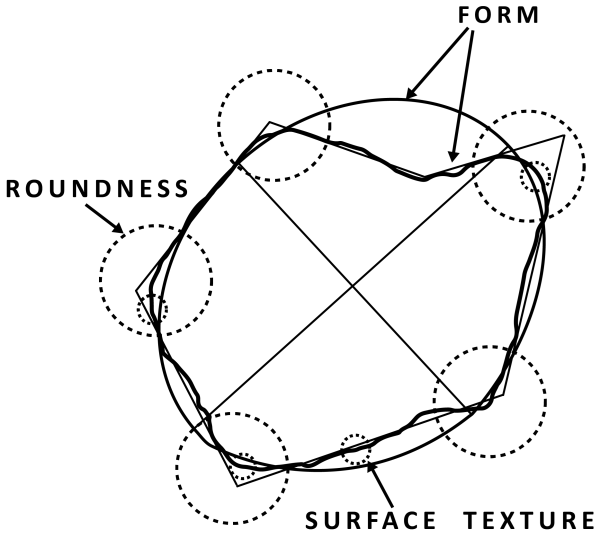
\includegraphics[scale=0.4]{fig1.png}}
\caption{Hierarchical order proposed by Barret. Features corresponding to irregularities of form, roundness, and surface texture.}
\label{fig1}
\end{figure}

Form describes the general appearance of the rock, it is a coarse sketch of contour. There are some expressions to measure form,  the most used, in the geological field, is the proposed by Wadell \cite{b6} which is obtained from the relationship between the radius of the circle whose area is equal to the particle and the radius of the smallest circle that inscribes the particle. Form is a well-established concept. On the other hand, roundness is a complex concept that is difficult to estimate. For this reason, we dedicate the present work to this parameter. To measure the degree of roundness, there are two approaches; those based on curvature \cite{b7} and those using frequency analysis \cite{b8}. The curvature-based method defines the degree of roundness as the ratio of the mean radius of curvature of the corners of a particle to the radius of the largest circumscribed circle possible. This method is simple and accurate, however it is a scale dependent method. The Fourier-based methods are invariant to scale, rotation and translation, however analyzing the spectrum is a complicated issue and of high computational cost \cite{b8}.

In this work, we propose to use neural networks to estimate the roundness of sedimentary rocks. The input variable to the neural network is the first component of principal components analysis (PCA) of the elliptical Fourier spectrum. The Fourier spectrum was chosen as the input variable because it is invariant to scale, rotation, and translation. The degree of roundness, calculated with the curvature method proposed by Wadell \cite{b6}, was used as the objective of the neural network. To calculate the roundness, we use the algorithm developed by Zheng and Hryciw \cite{b7}. The proposed neural network has the following architecture: 6-layer neural network, the input layer with 1000 neurons and Rectified Linear Unit (ReLU) activation function, 27 hidden layers with several different quantities of neurons each, with ReLU activation function. The output layer with a single neuron with a linear activation function. The database to train the neural network contains 1125 real-rocks images from some geological phenomena. The neural network model has a mean squared error of 6$E-4$ and a mean error of 6$E-3$. The neural network enables much faster processing. The roundness is estimated at 2800 times faster than the algorithm developed by Zheng and Hryciw. In addition, the method proposed is invariant to scale, rotation, and translation. Using a neural network we have combined the potentialities of the method based on curvature and frequency analysis.


\section{Materials and Methods}
In this section, we explain the concepts and mathematical expressions to estimate the roundness. The input variable to the neural network, elliptical Fourier, is described too.

\subsection{Roundness}
Roundness is a second-order property which is independent of the form. Roundness is related to the smoothness (or angularity) of particles. These variations are expressed in corners and edges. The degree of roundness can be estimated by two approaches: curvature and frequency contour analysis. Frequency analysis is described in section elliptical Fourier. The curvature approach was proposed Wadell\cite{b6}.  The curvature approach consists of finding the most significant curvatures in the contour. These curvatures are associated with the angularity of the particle. The smaller radius of curvature, the greater corner angle.  The more significant curvatures there are, the more angular the contour will be. An example is shown in Fig.~\ref{fig2}.
Roundness is a second-order property which is independent of the form. Roundness is related to the smoothness (or angularity) of particles. These variations are expressed in corners and edges. The degree of roundness can be estimated by two approaches: curvature and frequency contour analysis. Frequency analysis is described in section elliptical Fourier. Wadell's procedure \cite{b6} consists of finding the corners and fitting of circles to them. The concept is clear; however the algorithm to estimate this roundness is not easy to implement. Zheng and Hryciw \cite{b7} developed an algorithm which has four main steps: (1) find the maximum inscribed circle, (2) noise reduction, (3) identify the corners, and (4) fit circles to the corners. An example is shown in Fig.~\ref{fig2}.


\begin{figure}[htbp]
\centerline{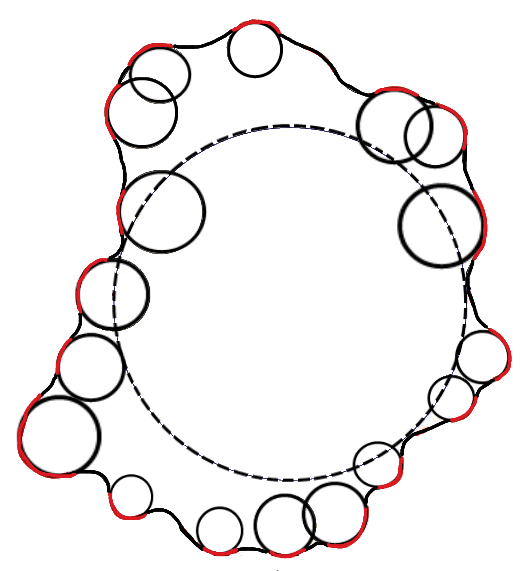
\includegraphics[scale=0.4]{fig2.png}}
\caption{Illustration of the method, proposed by Wadell, to measure the degree of roundness. The circle dotted line corresponds to maximum inscribed circle and the circles solid line correspond to main corners.}
\label{fig2}
\end{figure}

The maximum inscribed circle is used to normalize. This fact is important because the maximum circumscribed circle can be used to normalize.  Thus the degree of roundness of a corner can be expressed as $r_{n}/R$, where $r_{n}$ is the radius of curvature of the corner $n$ and $R$ is the radius of the maximum circumscribed circle. Wadell \cite{b6} expressed the total roundness of a particle as

\begin{equation}
D_{g} = \sum_{n=0}^{N-1}{ \frac{r_{n}}{R}}, \label{eq1}
\end{equation}

\noindent where $ N $ is the number of total corners in the contour. In this way, the range of roundness is between 0 and 1, being 0 a contour without corners (perfect circle) and 1 a contour with the possible maximum number of corners. The algorithm works properly, however, the threshold to identify between corners and non-corners depends on the scale. An inappropriate value, for this threshold, can lead to a considerable error.


\subsection{Elliptic Fourier}

Frequency analysis consists in obtaining the Fourier transform of the contour. In frequency, the three morphological characteristics are divided into frequency ranges. The low-frequency range is related to form, the medium-frequency range to roundness, and the high-frequency to roughness \cite{b8}. However, determining the limits of different morphological orders is not an easy task. It has been an unsolvable problem since the method was first proposed. To date, these limits are obtained empirically, with high uncertainty.


Because the particle contour is closed, elliptical Fourier is used. The elliptical Fourier method was proposed by Kuhl \cite{b9} which consists in obtaining the Fourier coefficients directly from the chain code of the contour. The chain code approximates the contour by a sequence of lines consisting of eight directions, Fig.~\ref{fig3}.

\begin{figure}[htbp]
\centerline{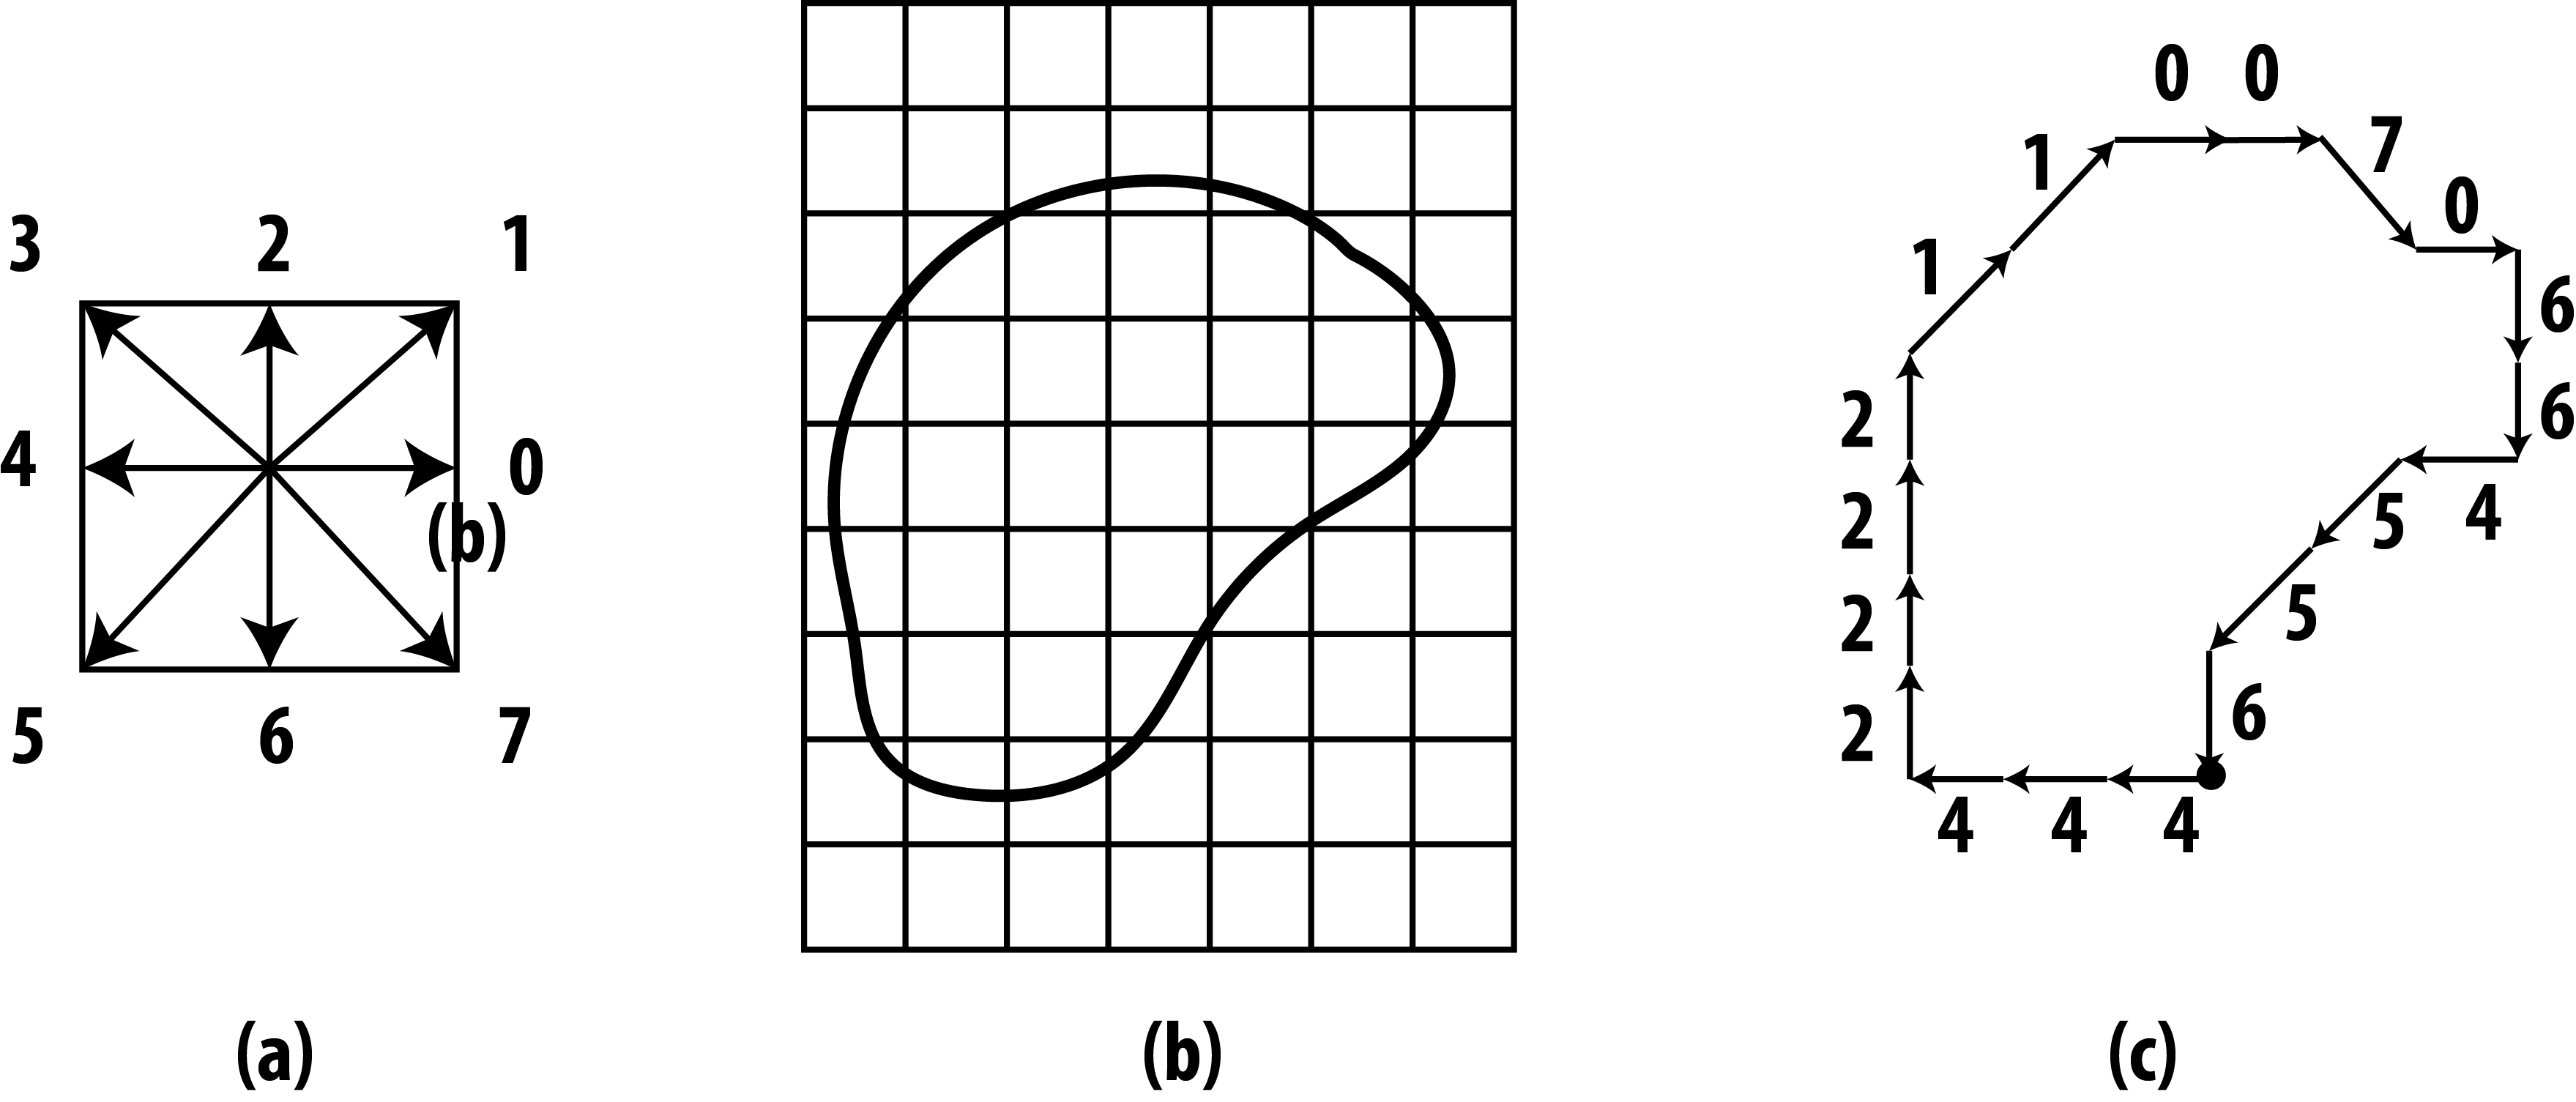
\includegraphics[scale=0.6]{fig3.png}}
\caption{Chain code. (a) Directions, (b) closed contour y (c)  chain elements. The dot indicates the chain start whose result is 4442222110070664556.}
\label{fig3}
\end{figure}

Chain code can be expressed in two coordinates; $x$ y $y$ axis, so the elements $x$ and $y$ of the chain are independent.  The expressions for the Fourier coefficients of the component \(x\) are

\begin{equation}
a_n = \frac{T}{2n^2\pi^2}\sum_{p = 1}^{K}\frac{\Delta x_p}{\Delta t_p}[\cos{\frac{2n\pi t_p}{T}} - \cos{\frac{2n\pi t_{p-1}}{T}}], \label{eq2}
\end{equation}

\begin{equation}
b_n = \frac{T}{2n^2\pi^2}\sum_{p = 1}^{K}\frac{\Delta x_p}{\Delta t_p}[\sin{\frac{2n\pi t_p}{T}} - \sin{\frac{2n\pi t_{p-1}}{T}}], \label{eq3}
\end{equation}

\noindent where, $K$ is the number of pixels of contour, \(T\) the fundamental period, \(\Delta x_p\) incremental change on the $x$ axis, \(\Delta t_p\) time incremental change. In a similar way, the coefficients of the component \(y\) are calculated by the following expressions

\begin{equation}
c_n = \frac{T}{2n^2\pi^2}\sum_{p = 1}^{K}\frac{\Delta y_p}{\Delta t_p}[\cos{\frac{2n\pi t_p}{T}} - \cos{\frac{2n\pi t_{p-1}}{T}}], \label{eq4}
\end{equation}

\begin{equation}
d_n = \frac{T}{2n^2\pi^2}\sum_{p = 1}^{K}\frac{\Delta y_p}{\Delta t_p}[\sin{\frac{2n\pi t_p}{T}} - \sin{\frac{2n\pi t_{p-1}}{T}}], \label{eq5}
\end{equation}

These four series of coefficients can be expressed by circular phasors, one for each axis; however, they can be drawn by a single elliptical phasor, hence its name. The invariance to scale, rotation, and translation are reached by normalization and rotation of angle of the first ellipse to zero, the expressions to achieve this can be consulted in \cite{b9}. The elliptical Fourier is two dependent spectra. Dependence complicates the delimitation of frequency ranges corresponding to form and roundness.

  
\subsection{Using deep neural networks to determine form and roundness}\label{AA}

A neural network is a type of machine learning which simulates the human learning mechanism. The neuron is the basic unit. A neural network contains a large number of neurons connected to each other. The connection between the neurons is known as synapse and its strength is determined by an external stimulus. In the artificial and biological neural network, the change in synaptic weight enables learning. The stimulus in artificial neural networks is provided by the training data containing input-output pairs of the function to be learned \cite{b10}. Neuron should be activated or not depending on whether it is relevant to the prediction. The function that performs this process is known as the activation function. The neural network is organized in layers. A layer consists of several neurons and has a specific order in relation to the others. The first layer receives the input data, the last layer provides the result. The intermediate layers are called hidden layers \cite{b11}.


\begin{figure}[htbp]
	\centerline{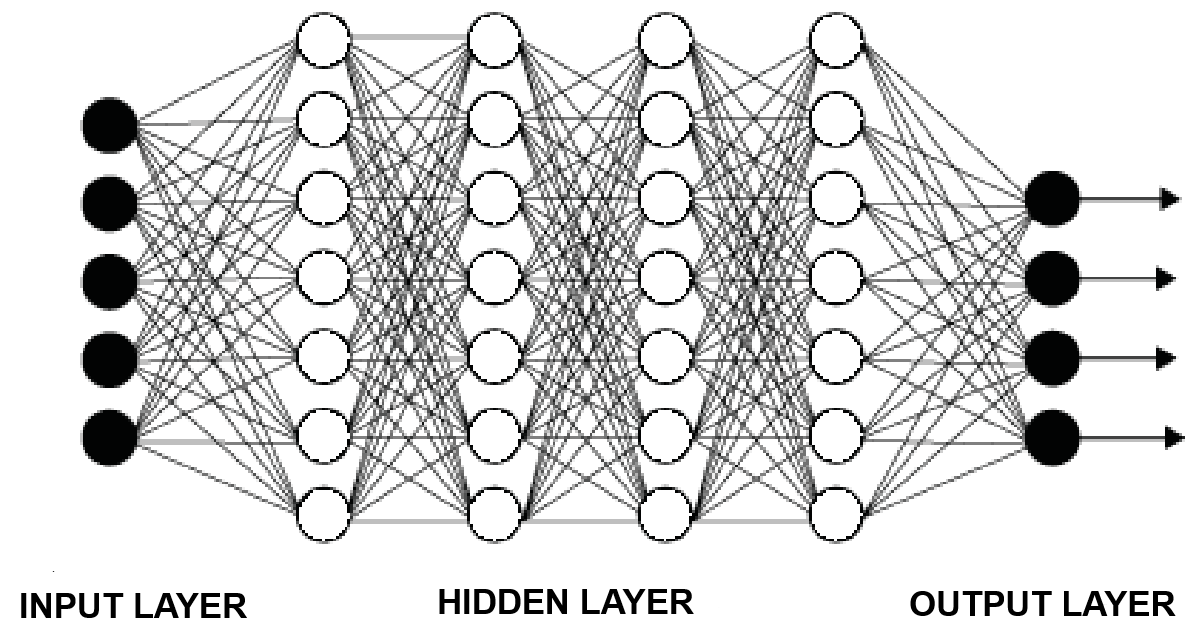
\includegraphics[scale=0.6]{fig4.png}}
	\caption{Typical structure neural network.}
	\label{fig4}
\end{figure}

A deep neural network consists of calculations carried out by many layers. Fig.~\ref{fig4} shows a deep neural network architecture with 4 hidden layers. The nodes of a layer are connected to the nodes of the previous and next layer. These types of networks are used to adjust complex models that requires a more sophisticated estimation \cite{b12}.

To link curvatures and frequency approaches, we proposed using deep neural networks to estimate the roundness of sedimentary rocks. The input variable to the neural network is PC 1 of the elliptical Fourier magnitude spectrum. We chose the spectrum as the input variable because it is invariant to scale, rotation, and translation. PCA was applied to reduce the dimensionality of the spectra resulting from elliptical Fourier. The degree of roundness obtained by the radius of the curvature (method described above) is used as the target value.

\section{Results and Discussion}
To explain the methodology used, Fig.~\ref{fig5} sketches the flow diagram of the proposed method.

\begin{figure}[htbp]
\centerline{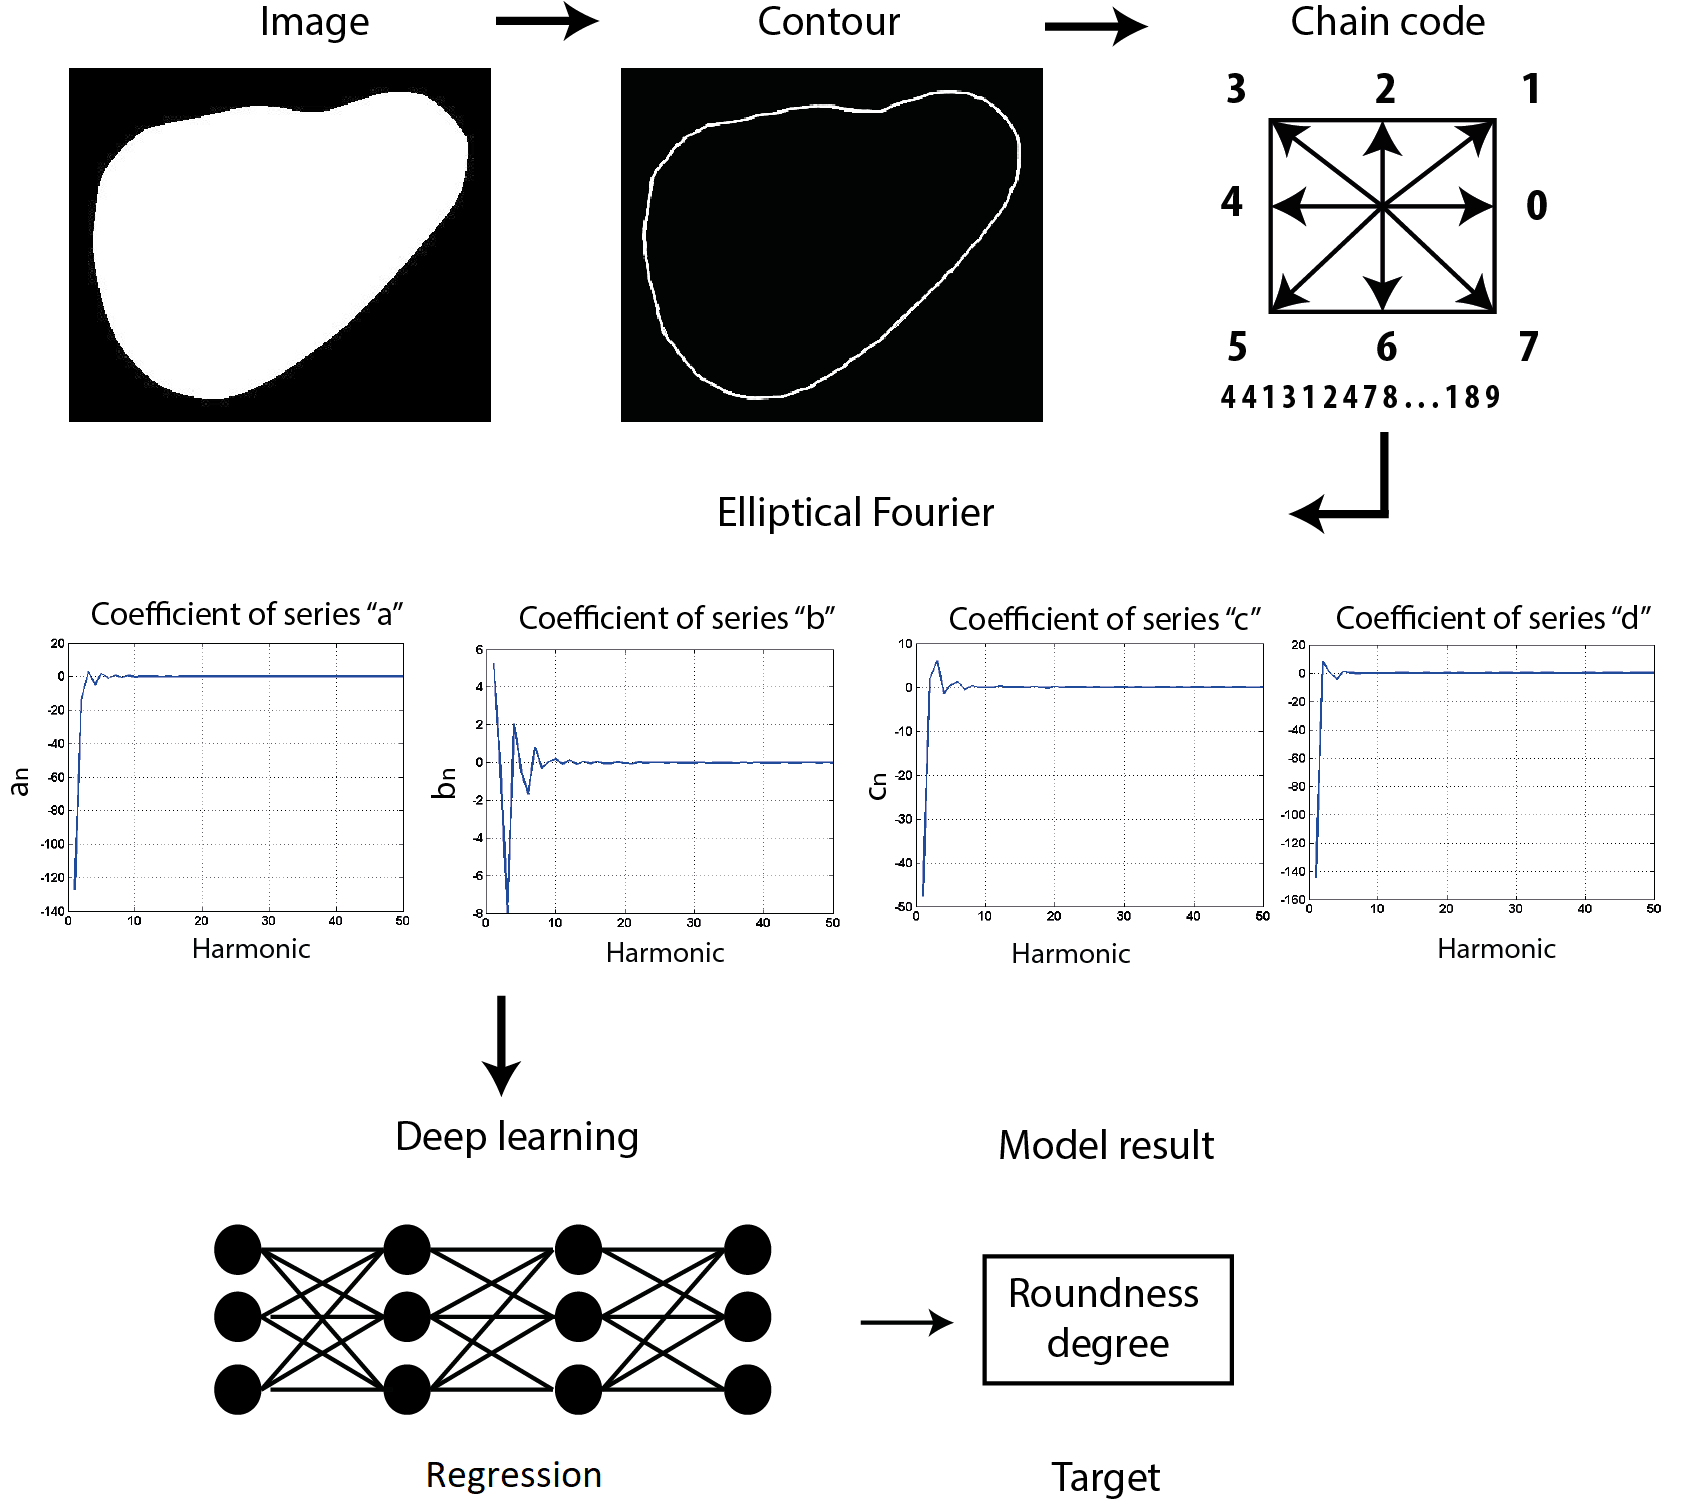
\includegraphics[scale=0.6]{fig5.png}}
\caption{Flow-chart of the developed method to measure the roundness of sedimentary rocks}
\label{fig5}
\end{figure}

The database to train and test the deep neural network was built from 1125 images of real rocks. The rocks analyzed correspond to pyroclastic falls, block and ash flow, debris avalanche and lahars. The database is available at https://github.com/Gamalielmch/DNN\textunderscore roundness.git.

\begin{figure}[htbp]
	\centerline{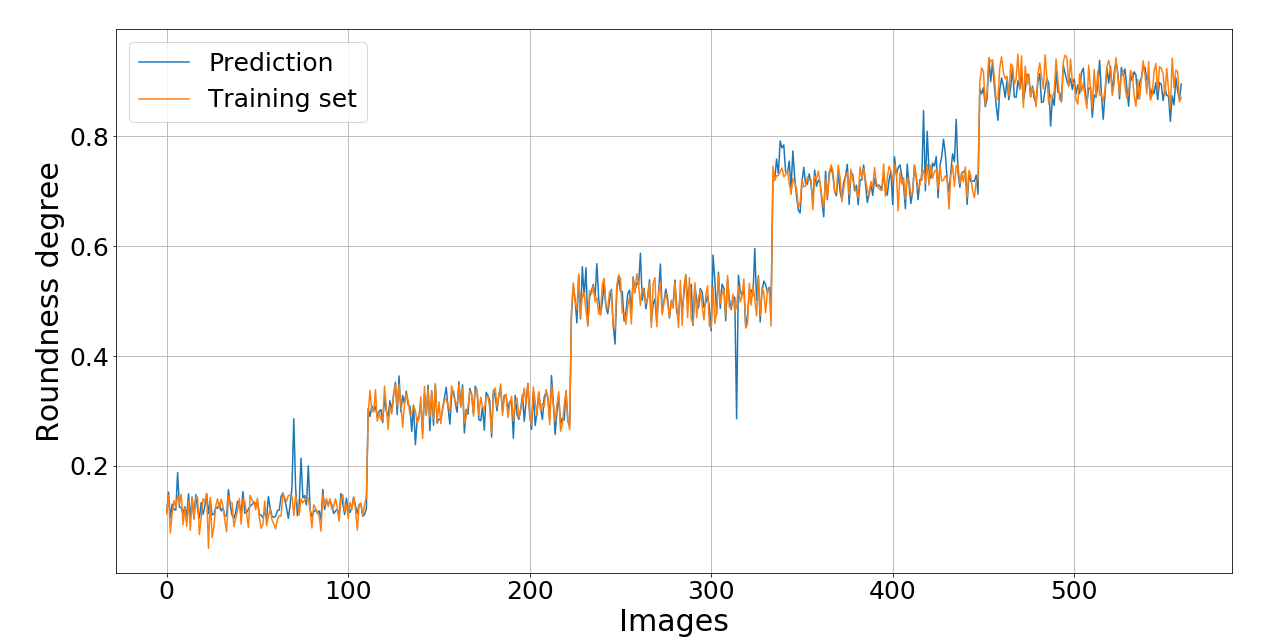
\includegraphics[scale=0.3]{fig6.png}}
	\caption{Result of deep neural network training}
	\label{fig6}
\end{figure}

Results of analysis reveal that the deep neural network with 29 layers, single input and output layer and twenty seven hidden layers, is the most appropriate architecture. The input layer with 1000 neurons with ReLU activation function, 27 hidden layers with several queantities of neurons each with ReLU activation function and the output layer with a single neuron with activation function linear is the most appropriate approach to measure roundness dregree. 

The ReLU activation function was chosen for hidden layers because the gradient of the Sigmoid and the TanH function can disappear with each iteration, which would affect the error propagation. The output layer consists of single neuron with linear activation function because the degree of roundness is a real number. Deep neural network training was performed in Python v3.7.3 using the Jupyter Notebook v5.7.8 platform, using the keras and sklearn libraries \cite{b13}. The result of the training is shown in Fig.~\ref{fig6}.

\begin{figure}[htbp]
	\centerline{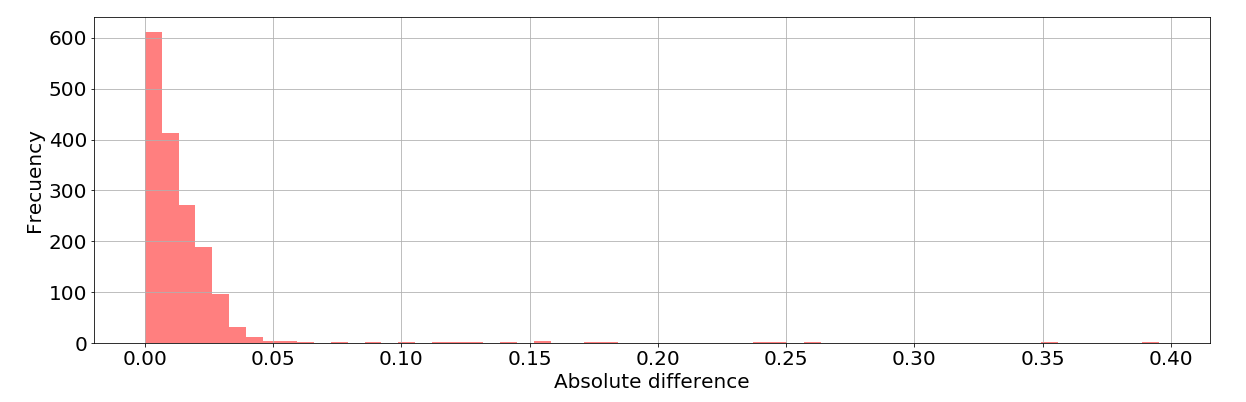
\includegraphics[scale=0.35]{fig7.png}}
	\caption{Absolute differences Histogram. Diference between the predicted value of the neural network and the roundness measured by the Zheng and Hryciw algorithm}
	\label{fig7}
\end{figure}


As can be seen from Fig.~\ref{fig6}, almost all model predictions simulate the roundness degree properly. The deep neural network has a mean squared error (MSE) of 6$E-4$ and a mean error of 6$E-3$. For more detail, the histogram of absolute difference is shown in Fig.~\ref{fig7}. The 98\% shows a difference of less than 0.05 and 79 \% of less than 0.02.

\begin{figure}[htbp]
	\centerline{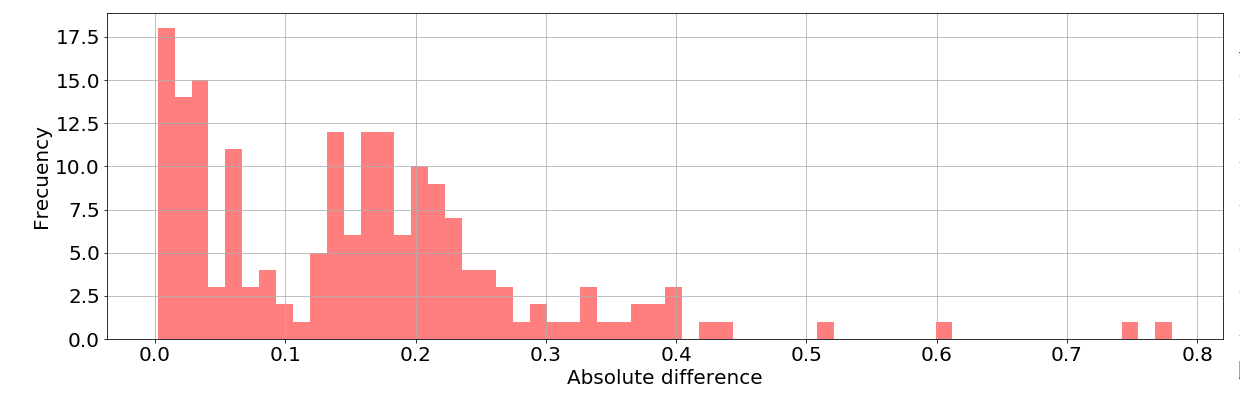
\includegraphics[scale=0.35]{fig8.png}}
	\caption{Absolute differences Histogram. Diference between the predicted value of the neural network and the roundness measured by the Zheng and Hryciw algorithm}
	\label{fig8}
\end{figure}

To test the deep neural network we have reserved a set of 180 images from the database which were chosen randomly. Fig.~\ref{fig9} shows the results of estimation for test set. The MSE is 0.041 and mean error is 0.016.


The fitting of the deep neural network is  is accurate for 98\% of cases, since a difference of less than 0.05 is very acceptable in geological studies. However, Fig.~\ref{fig8} shows the lack to predict new examples, with only 26\% below of 0.05.

\begin{figure}[htbp]
\centerline{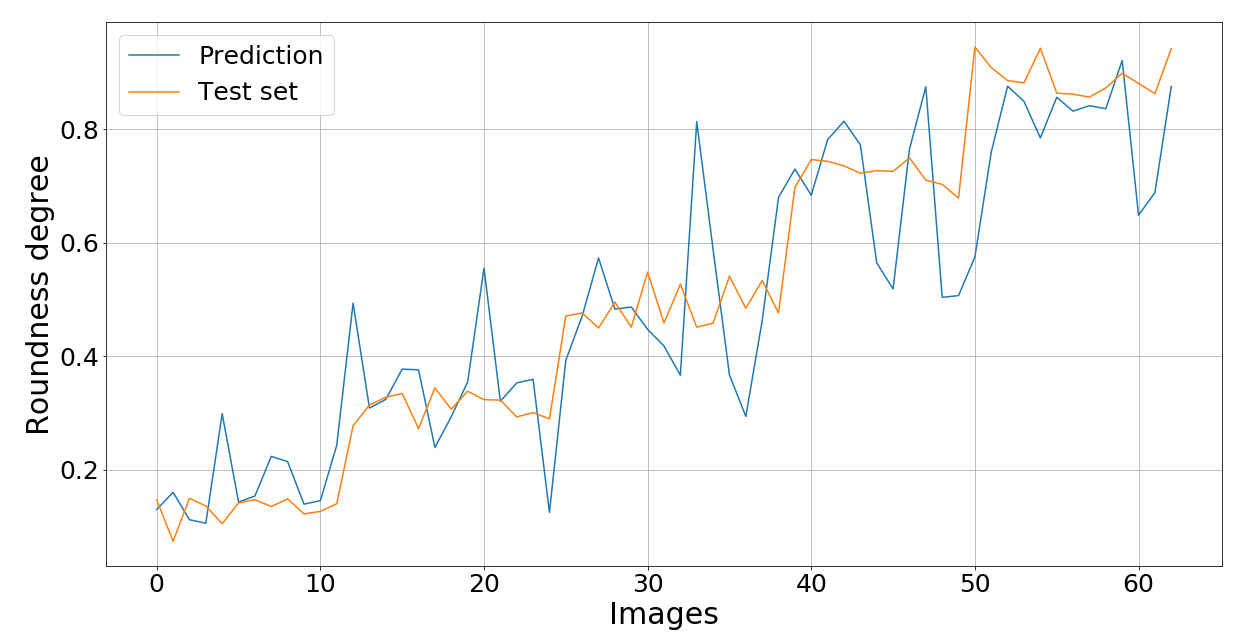
\includegraphics[scale=0.3]{fig9.png}}
\caption{Result of deep neural network for test set}
\label{fig9}
\end{figure}

\section{Conclusions}
This work describes the implementation of a deep neural network to estimate the roundness of sedimentary rocks. We use two approaches, curvature and frequency analysis. The input data are the 6 to 50 coefficients of elliptical Fourier and the target data are the curvature of the main corners of the contour. Using these two approaches, we developed an invariant method to scale, rotation, and translation. Based on several architectures, it is concluded that the deep neural network with 28 layers, with several different quantities of neurons, is the most appropriate to prediction roundness degree. 

The deep neural network was trained and tested using 1125 images of real rocks from some geological phenomena. The fitting of the network shows that 91 \% of the training data have a difference of less than 0.05. On the other hand, the MSE of the test data was 0.0011 and the mean error was 0.019, a highly acceptable difference in the geological field. The deep neural network model, proposed in this manuscript, can be easily used by readers. The model is freely distributed and available in the repository https://github.com/Gamalielmch/DNN\textunderscore roundness.


% use section* for acknowledgment
\section*{Acknowledgments}

The Author also extends thanks to Conacyt for Retention Grant No. 2019-000010-01NACV-00020 and support the project No. ZAC-2018-05-125266. 

	
\begin{thebibliography}{plain}
\bibitem{b1} S. jr. Boggs, ``Petrology of sedimentary rocks,'' Cambridge: Cambridge University Press., vol. III, 2013.
\bibitem{b2} J. M. Rodriguez, T. Edesk{\"{a}}r and S. Knutsson, ``Particle shape quantities and measurement techniques-A review,'' Electronic Journal of Geotechnical Engineering, vol. 18a,pp.169--198, 2013.
\bibitem{b3} M. E. Tucker, ``Sedimentary petrology: an introduction to the origin of sedimentary rocks,''John Wiley \& Sons, 2009.
\bibitem{b4} M. Diepenbroek, A. Bartholom{\"{a}}, and I. Hillert, ``How round is round? A new approach to the topic  roundness by Fourier grain shape analysis,'' Sedimentology. pp. 411--422, 1992.
\bibitem{b5} P. J. Barrett, ``The shape of rock particles, a critical review,'' Sedimentology, vol. 27, pp. 291--303, 1980.
\bibitem{b6} H. Wadell, ``Volume, shape, and roundness of rock particles,'' The Journal of Geology, vol. 40, pp. 443--451, 1932.
\bibitem{b7} J. Zheng and R. D. Hryciw, ``Particle roundness and sphericity from images of assemblies by chart estimates and computer methods,'' Journal of Geotechnical and Geoenvironmental Engineering, vol. 142, pp. 1--15, 2016.
\bibitem{b8} I. Charpentier,  D. Sarocchi  and L. A. Rodriguez, ``Particle shape analysis of volcanic clast samples with the Matlab tool MORPHEO,'' Computers and Geosciences, vol. 51, pp. 172--181, 2013.
\bibitem{b9} F.P. Kuhl and C. R. Giardina, ``Elliptic Fourier features of a closed contour,'' Computer Graphics and Image Processing, vol. 18, pp. 236--258, 1982.
 \bibitem{b10} Charu C. Aggarwal, ``Neural Networks and Deep Learning,'' Materials \& design 28.6 (2007): 1747-1752.
\bibitem{b11} W. Sha and K. L. Edwards, ``The use of artificial neural networks in materials science based research,'' Materials \& design 28.6 (2007): 1747-1752.
\bibitem{b12} M.A. Nielsen, ``Neural networks and deep learning,'' Determination Press, 2015.
\bibitem{b13} J. Moolayil. ``Learn Keras for Deep Neural Networks,'' Apress, 2019.

\end{thebibliography}

% that's all folks
\end{document}


